\documentclass[thesis.tex]{subfiles}
\def\x{\mathbf{x}}
\def\y{\mathbf{y}}
\def\d{\mathbf{d}}
\def\c{\mathbf{c}}
\begin{document}
\chapter{Proposed descriptor}
%
Given a region centered at a point $\x_0$ in an image at scale $\sigma_0$, we wish to effectively describe the region. Our proposed descriptor consists of weighted kernel-based histograms, explained in \Cref{sec:histograms}, computed for $m$ \textit{cells} arranged in a grid. We define the $j$'th cell histogram $H_j$ as
%
\begin{align}
\label{eq:proposed_histogram}
H_j(f_i) = \int F(\x) A_j (\x) P (\x) B(\x; f_i,f) \,\text{d} \x
\end{align}
%
where
%
\begin{itemize}
\item[] $f_i$ for $i = 1 \dots n$ are bin centers,
\item[] $f$ is a bin value function on the domain $[f_\text{min},f_\text{max}]$,
\item[] $F$ is a magnitude function,
\item[] $A_j$ for $j = 1 \dots m$ are cell aperture functions,
\item[] $P$ is a center aperture function, and
\item[] $B$ is a binning aperture function.
\end{itemize}
%
We will use the above terminology throughout this chapter. Note that we have kept this definition similar to the galaxy descriptor \cite{pedersen2013shape}, except we consider several histograms with their own aperture functions $A_j$ and add the additional center aperture function $P$. The descriptor $\d$ is constructed by concatenating all $n$ bin values of all $m$ cell histograms:
%
\begin{align}
\label{eq:proposed_descriptor}
\d = \Bigl( \left(H_1(f_1) \cdots H_1(f_n)\right) \cdots (H_m(f_1) \cdots H_m(f_n)) \Bigr) ^\text{T}
\end{align}
%
The five functions above can be seen as the components that make up our descriptor, and we consider different choices for each. The functions depend on numerous additional parameters, which we define and describe throughout this chapter. Most of these parameters will be subject to a parameter study for each of our applications in order to find the optimal descriptor for the specific application. The parameter studies are described in \Cref{sec:icParameterStudy,sec:odParameterStudy}. After describing the descriptor parameters, we show a detailed example of the descriptor being computed for an image.
%
\section{Bin value and magnitude functions}
\label{sec:valueMagnitudeFunctions}
%
The choice of bin value and magnitude functions are closely connected, as we wish the magnitude function to weight the histogram values according to their importance for the local image structure. By far the most common choice in literature \cite{lowe2004distinctive,ke2004pca,mikolajczyk2005performance,tola2008fast} is using gradient orientation $\Theta$ as value function and gradient magnitude $M$ as magnitude function. Another good choice from the galaxy descriptor \cite{pedersen2013shape} is to use shape index $S$ weighted by curvedness $C$. Finally we have experimented with the $l,b,a$ re-parametrization of second order information weighted by 2-jet norm $\| \mathbf{j} \|$ \citep{griffin2007second}. This was however unable to produce good results through initial testing, and we decided not to pursue the idea further.

Our strategy is thus to create a descriptor based on $\Theta$ and $M$ (referred to as GO), one based on $S$ and $C$ (referred to as SI), as well as a concatenation of these descriptors (referred to as GO+SI). These functions are defined in \Cref{sec:gradientTheory,sec:shapeIndexTheory}.

Recall that in order to make our descriptor scale invariant, we wish to compute the descriptor according to the scale $\sigma_0$ of its region center $\x_0$. This is achieved by computing a scale space pyramid of both value and magnitude images across all region scales. The values and magnitudes needed to compute the cell histograms can then be found by lookup in these scale space images. Before making this lookup, we propose a pre-processing step on the magnitude images to make our descriptor robust to local illumination changes.
%
\subsection{Local magnitude normalization}
\label{sec:localMagnitudeNormalization}
%
In \Cref{sec:illumination} we described the problem of handling illumination in images and its possible solutions. The block-normalization scheme from the HOG descriptor \cite{dalal2005histograms} is a way of locally (in blocks of $2 \times 2$ cells) estimating the affine coefficient $a$ when having assumed an affine illumination model. \todo{reference?} We wish to make this estimation even more local by estimating $a$ on a pixel-level. We propose a normalization scheme called pixel-wise normalization, which we apply to the magnitude function $F(\x)$.
The pixel-wise normalized magnitude at a point is defined as the magnitude relative to a local area, which we compute by convolution with a Gaussian filter:
%
\begin{align}
F_\text{norm}(\x) = \frac{F(\x)}{\int F(\y) G(\y - \x; \eta \sigma_0) \,\text{d} \y}
\end{align}
%
where $\eta$ is the normalization scale, defined relative to the region scale $\sigma_0$. The idea behind this scheme is that an image is locally affected by light changes according to the affine illumination model. In order to estimate $a$ on a pixel-level, we use intensity information from the surrounding pixels. Using a Gaussian filter we are able to weight the surrounding intensities based on their spatial distance to the pixel in question. The rationale for this is, that pixels close to one another has a higher probability of being affected by equal light conditions than pixels further away from one another. By dividing the pixel value by the sum of all these weighted intensities (estimation of $a$), we remove the affine coefficient from the pixel.

Having applied the pixel-wise normalization to the magnitude scale space images we are done pre-processing the images and able to perform lookups of values and magnitudes for each region.
\Cref{fig:pixelNormalizationExample} shows two examples of images containing shadows, their gradient magnitudes at $\sigma_0 = 1$, their pixel-wise normalized magnitudes with $\eta = 2$, and their pixel-wise normalized magnitudes with $\eta = 10$. These types of shadows are the ones we will try to handle by using pixel-wise normalization. As seen in the gradient magnitude images, the shadows have a dampening effect on the gradient magnitude. By using a small $\eta$ for the pixel-wise normalization, we see that a lot of the noise is enhanced but the shadows (especially the edges) are a lot less significant than for the normal gradient magnitudes. When using a larger $\eta$ the noise is smoothed out and less significant. Furthermore there seem to be more of the structure highlighted from within the area affected by the shadows, but the shadow edges are more significant as well. The choice of optimal $\eta$ is part of our parameter studies.

An alternative technique for handling local illumination is normalizing each cell histogram, which can be done instead of or alongside pixel-wise normalization. This was used successfully in the DAISY descriptor \cite{tola2008fast}. We have tried various ways of incorporating this technique, but none were able to beat simple pixel-wise normalization through preliminary tests, and hence we have refrained from pursuing these strategies further.
%
\begin{figure}[p]
    \centering
    \begin{subfigure}[t]{0.48\textwidth}
        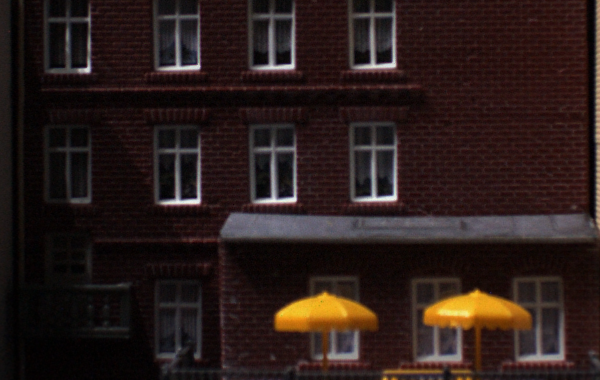
\includegraphics[width=\textwidth]{img/pixelNormalizationExample1.png}
        \caption{}
        \label{fig:pixelNormalizationExample1}
    \end{subfigure}
    \begin{subfigure}[t]{0.48\textwidth}
        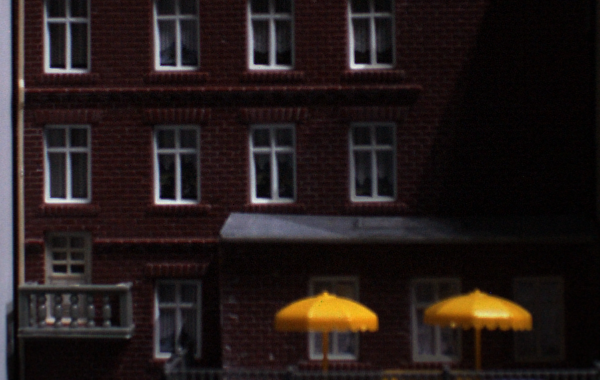
\includegraphics[width=\textwidth]{img/pixelNormalizationExample2.png}
        \caption{}
        \label{fig:pixelNormalizationExample2}
    \end{subfigure}
    \begin{subfigure}[t]{0.48\textwidth}
        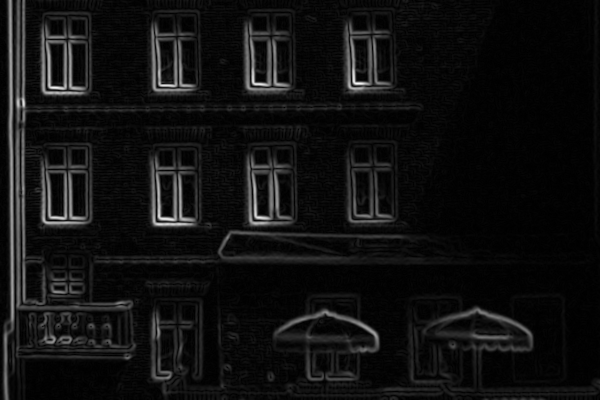
\includegraphics[width=\textwidth]{img/pixelNormalizationExample3.png}
        \caption{}
        \label{fig:pixelNormalizationExample3}
    \end{subfigure}
    \begin{subfigure}[t]{0.48\textwidth}
        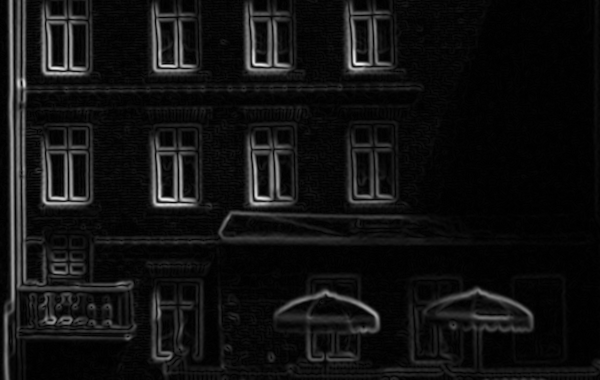
\includegraphics[width=\textwidth]{img/pixelNormalizationExample4.png}
        \caption{}
        \label{fig:pixelNormalizationExample4}
    \end{subfigure}
    \begin{subfigure}[t]{0.48\textwidth}
        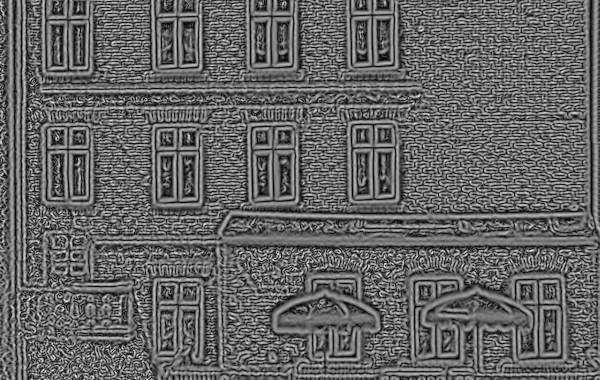
\includegraphics[width=\textwidth]{img/pixelNormalizationExample5.png}
        \caption{}
        \label{fig:pixelNormalizationExample5}
    \end{subfigure}
    \begin{subfigure}[t]{0.48\textwidth}
        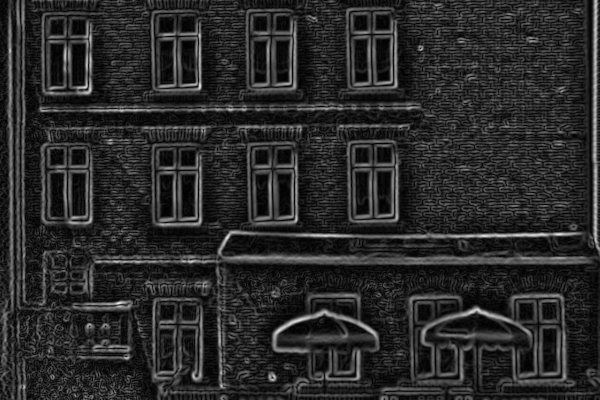
\includegraphics[width=\textwidth]{img/pixelNormalizationExample6.png}
        \caption{}
        \label{fig:pixelNormalizationExample6}
    \end{subfigure}
    \begin{subfigure}[t]{0.48\textwidth}
        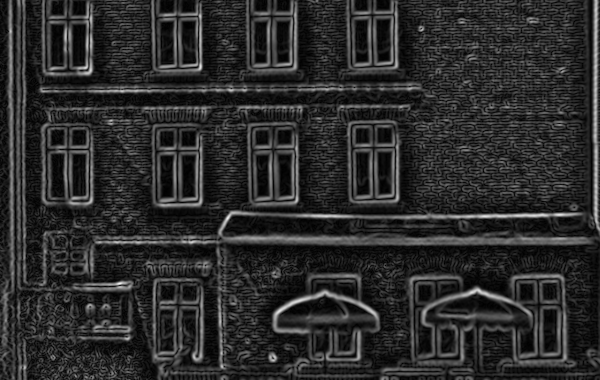
\includegraphics[width=\textwidth]{img/pixelNormalizationExample7.png}
        \caption{}
        \label{fig:pixelNormalizationExample7}
    \end{subfigure}
    \begin{subfigure}[t]{0.48\textwidth}
        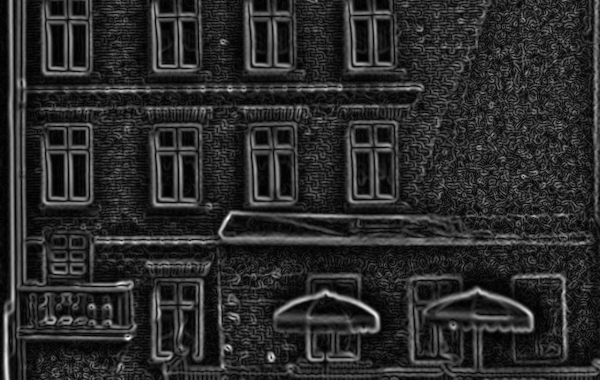
\includegraphics[width=\textwidth]{img/pixelNormalizationExample8.png}
        \caption{}
        \label{fig:pixelNormalizationExample8}
    \end{subfigure}
    \caption{Images \subref{fig:pixelNormalizationExample1} and \subref{fig:pixelNormalizationExample2} show cut-outs of an image with artificial lighting from the left and right, respectively. Images \subref{fig:pixelNormalizationExample3} and \subref{fig:pixelNormalizationExample4} show gradient magnitudes of these images. Images \subref{fig:pixelNormalizationExample5} and \subref{fig:pixelNormalizationExample6} show pixel-wise normalized magnitudes for normalization scale $\eta = 2$. Images \subref{fig:pixelNormalizationExample7} and \subref{fig:pixelNormalizationExample8} show pixel-wise normalized magnitudes for $\eta = 10$.}
    \label{fig:pixelNormalizationExample}
\end{figure}
%
\section{Cell aperture function}
\label{sec:cellApertureFunction}
%
The purpose of the cell aperture functions $A_j$ is to weight points closer to each cell center higher in their respective cell histograms. We define a cell aperture function as
%
\begin{align}
A_j(\x) = K(\x - (\x_0 + r \sigma_0 \c_j); \alpha k_j r \sigma_0),
\end{align}
%
where \todo{annoying cut-off}
%
\begin{itemize}
\item[] $K$ is a kernel function as described in \ref{sec:apertureKernelFunctions},
\item[] $\c_j$ is the relative cell center position for cell $j$,
\item[] $\alpha$ is the cell scale across all cells,
\item[] $k_j$ is a cell scale specific to cell $j$, and
\item[] $r$ is a radius parameter defined below according to the cell layout, scaling both cell scales and relative positions.
\end{itemize}
%
Note that the cell aperture function is simply a kernel function centered at each cell $j$ for a specific region center $\x_0$ and scaled according to the layout radius $r$ and region scale $\sigma_0$.

The cell aperture function is defined for all cells of the region. Having defined $A_j$ we are now able to define the \emph{cell layouts} that define the cell centers $\c_j$ for each region. The layouts depend on the application, and hence we split our proposed cell layouts into two categories: interest point and region layouts. \todo{Should we rename the region layouts?}

\subsection{Interest point cell layouts}
\label{sec:cellApertureFunctionPoint}
When describing an interest point the structure surrounding the interest point is of great importance. Interest points are usually found using a detector as described in \Cref{sec:interestPointDetectors}. The innermost cells of the cell layouts are therefore spatially smaller than the cells further away, in order to capture the structural variations close to the interest point in greater detail. Given the nature of the layouts as structured grids, we refer to them as \emph{grid types}.

\Cref{fig:gridType} shows examples of the six different grid types that we propose for describing the local area around an interest point: polar, polar central, log-polar, concentric polar, concentric polar central, and concentric log-polar. These layouts are inspired by the GLOH \cite{mikolajczyk2005performance}, Irregular SIFT \cite{cui2009scale}, and DAISY \cite{tola2008fast} layouts. Circular grids are chosen in order to retrieve an even amount of information around the interest point. The four polar grids use polar cell kernels, where points are converted from Cartesian coordinates into polar coordinates before applying the kernel. The two log-polar grids both use standard Cartesian kernels. The examples are shown for the \emph{grid size} $8 \times 2$ meaning that each layout has 8 cells in each of their 2 rings. The two ``central'' and log-polar grids additionally have a single central cell. The two types of cells are illustrated in \Cref{fig:gridWindow} for a Gaussian kernel.

All these layouts are defined relative to the \emph{grid radius} $r$ and interest point scale $\sigma_0$. In other words the grid radius defines the span of the feature. The grid types are defined such that by default the 1 standard deviation curves of the outer-most cells in the feature touch the grid radius. Each ring consists of $n$ cells dividing the ring equally in the angular direction. The cells have varying size depending on their position in the grid, and hence each cell $j$ has its 1 standard deviation defined by a cell scale parameter $k_j$ relative to $r$ and $\sigma_0$. The following holds for each of the specific grid types:

For log-polar grid types the radial span of each ring is defined such that the 1 standard deviation of each cell $j$ touches the 1 standard deviation curves of the neighbouring rings and neighbouring angles by default. This results in different default cell scales for the normal and concentric log-polar grid types, since the concentric log-polar grid type can pack the cells more densely without overlapping cells as seen in \Cref{fig:gridTypeLp,fig:gridTypeClp}.
For polar grid types the radial span is divided equally between the rings. The polar central grid types are furthermore having a central cell of half the radial span of the rings. The polar Gaussian cell aperture function combined with positioning of the cell centers $\c_j$ are shown in \Cref{fig:gridTypeP,fig:gridTypePc,fig:gridTypeCp,fig:gridTypeCpc}.
See \Cref{apx:gridLayouts} for more information on how to compute the grid type cell positions.

As mentioned in the descriptions above, the grids are defined with default cell scales. These cell scales can be scaled both up and down by varying $\alpha$ to allow for additional or less overlap between the cells. This will however not change the positioning of the cell centers $\c_j$.

For the grid type examples in this section, we have simply chosen a grid size and a grid radius. These two variables have a major impact on the dimensionality and final outcome of the descriptor along with the cell kernel and its scale $\alpha$, and hence these parameters are tuned in our parameter studies in order to get the optimal descriptor grid type and overlap.

\subsection{Region cell layouts}
\label{sec:cellApertureFunctionRegion}

The goal of a region cell layout is to describe a specified region of an image with no bias towards any reference point. These layouts are typically used in conjunction with a sliding window approach as described in \Cref{sec:slidingWindow}. The shape of the region depends on the application and dataset. Regions are specified by a central point $\x_0$ with scale $\sigma_0$ similar to the interest point layouts. Like the interest point cell layouts, the region cell layouts are structured in grids and hence we likewise refer to these as grid types.
\Cref{fig:gridTypeWindow} shows examples of the two grid types that we propose for describing rectangular regions: square and triangle.

By default the 1 standard deviations of neighbouring cells are tangent to each other. The size of the 1 standard deviation, and hence also the spacing of the cells, is defined as the cell spacing $r$. Following the logic from the interest point grid types, the 1 standard deviations can be scaled to allow for additional or less overlap between the cells using the cell scale parameter $\alpha$.
The layouts are however only defined for a limited region, which causes problems when using the grid types in practice. Upscaling\todo{Up-scaling?} the overlap changes the support radius of each cell, which means that some cells span outside the defined region. In order to avoid this problem, we define another scaling parameter $k_j$ for each cell $j$. For cells with support radius inside the defined region, we define $k_j = 1$. For the remaining cells we define $k_j$ such that the support radius of each cell is tangent to the closest region boundary.
By increasing $\alpha$, the boundary cells will therefore keep their original scale defined by $r$, whereas the cells further away from the boundary will have increased overlap.
%
\begin{figure}[p]
	\centering
	\begin{subfigure}[t]{\textwidth}
		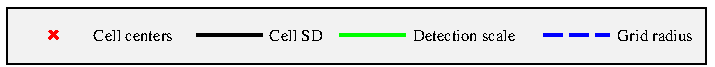
\includegraphics[width=\textwidth]{img/gridType_legend.pdf}
	\end{subfigure}
	\begin{subfigure}[t]{0.32\textwidth}
		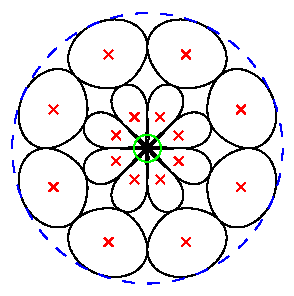
\includegraphics[width=\textwidth]{img/gridType_polar_polar_gaussian.pdf}
		\caption{Polar (P)}
		\label{fig:gridTypeP}
	\end{subfigure}
	\begin{subfigure}[t]{0.32\textwidth}
		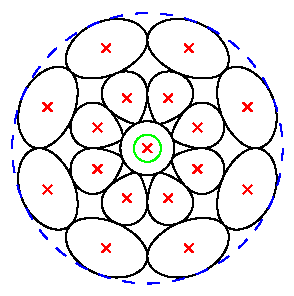
\includegraphics[width=\textwidth]{img/gridType_polar_central_polar_gaussian.pdf}
		\caption{Polar central (PC)}
		\label{fig:gridTypePc}
	\end{subfigure}
	\begin{subfigure}[t]{0.32\textwidth}
		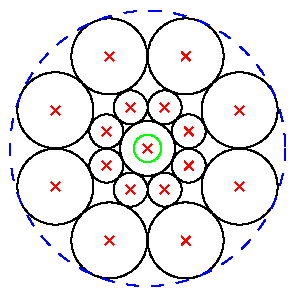
\includegraphics[width=\textwidth]{img/gridType_log-polar.pdf}
		\caption{Log-polar (LP)}
		\label{fig:gridTypeLp}
	\end{subfigure}
	\begin{subfigure}[t]{0.32\textwidth}
		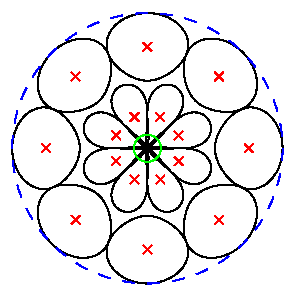
\includegraphics[width=\textwidth]{img/gridType_concentric_polar_polar_gaussian.pdf}
		\caption{Concentric polar (CP)}
		\label{fig:gridTypeCp}
	\end{subfigure}
	\begin{subfigure}[t]{0.32\textwidth}
		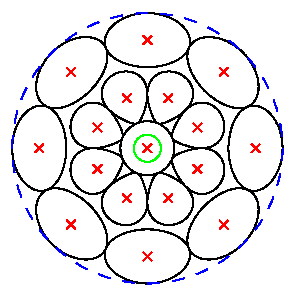
\includegraphics[width=\textwidth]{img/gridType_concentric_polar_central_polar_gaussian.pdf}
		\caption{Concentric polar central (CPC)}
		\label{fig:gridTypeCpc}
	\end{subfigure}
	\begin{subfigure}[t]{0.32\textwidth}
		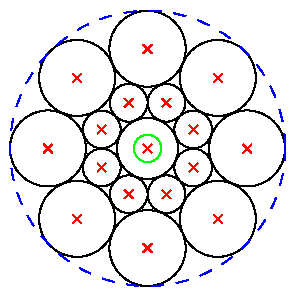
\includegraphics[width=\textwidth]{img/gridType_concentric_log-polar.pdf}
		\caption{Concentric log-polar (CLP)}
		\label{fig:gridTypeClp}
	\end{subfigure}
	\caption{Examples of cell grid types centered around a detected interest point, showing cell centers, 1 standard deviation curves (see \Cref{fig:gridWindow}), detection scales, and grid radii. The grid size here is $8 \times 2$ (8 cells in each of 2 rings) and the grid radius $r$ is set to 10, which is relative to the detection scale. The polar grids utilize polar Gaussian aperture cell functions while the log-polar use Cartesian Gaussian aperture cell functions.}
	\label{fig:gridType}
	\vspace{5mm}
		\begin{subfigure}[t]{\textwidth}
		\centering
		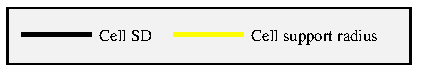
\includegraphics[width=0.5\textwidth]{img/cellWindow_legend.pdf}
	\end{subfigure}
	\begin{subfigure}[t]{0.40\textwidth}
		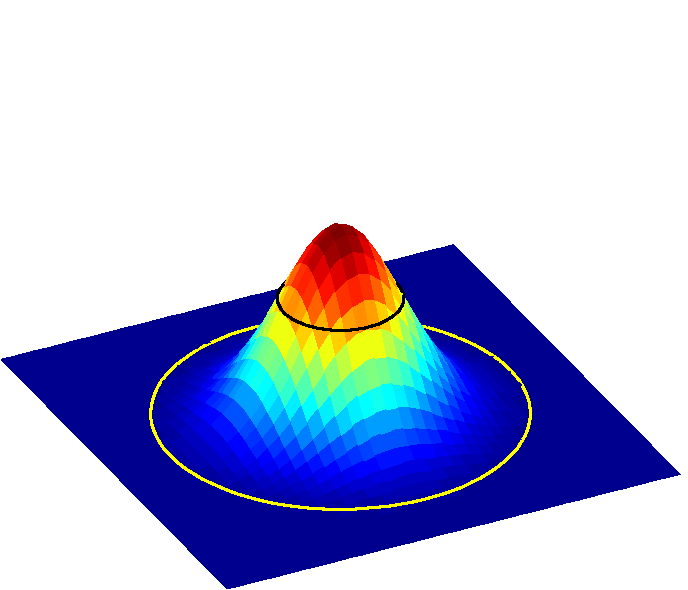
\includegraphics[width=\textwidth, clip=true, trim=0 0 0 90]{img/cellWindow.pdf}
		\caption{Gaussian}
		\label{fig:cellWindow}
	\end{subfigure}
	\begin{subfigure}[t]{0.40\textwidth}
		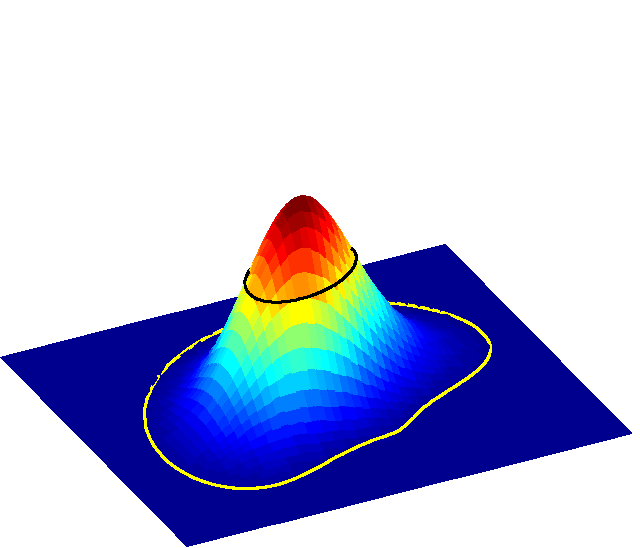
\includegraphics[width=\textwidth, clip=true, trim=0 0 0 90]{img/cellWindowPolar.pdf}
		\caption{Polar Gaussian}
		\label{fig:cellWindowPolar}
	\end{subfigure}
	\caption{The two types of Gaussian cell aperture functions plotted in 3D. The black curves are placed 1 standard deviation $\alpha$ from the cell centers. The yellow curves are placed $3 \alpha$ from the cell centers and confine the regions used to compute the cell histograms.}
	\label{fig:gridWindow}
\end{figure}
%
\begin{figure}[tb]
	\centering
	\begin{subfigure}[t]{\textwidth}
		\centering
		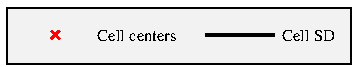
\includegraphics[width=0.5\textwidth]{img/gridType_legend_cropped.pdf}
	\end{subfigure}
	\begin{subfigure}[t]{0.45\textwidth}
		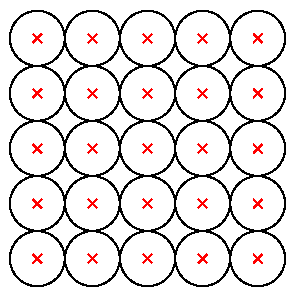
\includegraphics[width=\textwidth]{img/gridType_square_window.pdf}
		\caption{Square grid}
		\label{fig:gridTypeSquare}
	\end{subfigure}
	\begin{subfigure}[t]{0.45\textwidth}
		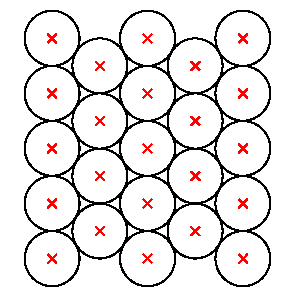
\includegraphics[width=\textwidth]{img/gridType_triangle_window.pdf}
		\caption{Triangular grid}
		\label{fig:gridTypeTriangle}
	\end{subfigure}
	\caption{Examples of region cell layout grid types used for sliding windows, where we are interested in describing a larger area rather than the local area surrounding a detected point.}
\label{fig:gridTypeWindow}
\end{figure}
%
\section{Center aperture function}
\label{sec:centerApertureFunction}
%
Similarly to $A_j$, the purpose of the center aperture function $P$ is to weight points closer to the detected interest point higher, since they are of greater importance to the local structure. The function is thus omitted for region descriptors. We define it as
%
\begin{align}
P(\x) = K(\x - \x_0; \rho r \sigma_0)
\end{align}
%
where $K$ is a kernel function as described in \ref{sec:apertureKernelFunctions}, and $\rho$ is the scale of the center aperture function. When $\rho = 1$, the standard deviation of the center aperture function is equal to the grid radius scaled by the detection scale. This function is inspired by SIFT \cite{lowe2004distinctive} and DAISY \cite{tola2008fast}\todo{Should we remove the references?} which use a similarly defined center aperture function. For SIFT the standard deviation of the corresponding function is pre-defined to have a scale half its square-grid width and height, whereas we search for the optimal $\rho$ by adding it to our parameter studies.\todo{What is $\rho$ for DAISY?}
%
\section{Binning aperture function}
\label{sec:binningApertureFunction}
%
The binning aperture function decides the shape of the histograms that make up our descriptor. We define it as
\begin{align}
	B(\x; f_i, f) = K \left( f(\x) - f_i; \beta \frac{f_\text{max} - f_\text{min}}{2n} \right)
\end{align}
where $K$ is a kernel function as described in \ref{sec:apertureKernelFunctions}, and $\beta$ is the bin scale, defined relative to a uniform bin layout. That is, when $\beta = 1$, the standard deviations of each bin are tangent to neighbouring bins.

For our proposed descriptors the value function $f$ is either the gradient orientation or the shape index. The number $n$ of bin centers $f_i$ for $i = 1,\hdots,n$ is variable and hence we need to define the bin centers as a function of $n$. Given an interval $[f_\text{min},f_\text{max}]$, we define the bin centers $f_i$
\begin{align}
	\label{eq:binCenters}
	f_i &= f_\text{min} + \frac{f_\text{max}-f_\text{min}}{n} \left(i - \frac{1}{2} \right)
\end{align}
which corresponds to splitting the interval into $n$ equally sized parts and placing the bin centers $f_i$ in each of the $n$ centers of these parts.

The shape index has values spanning the interval $[-1,1]$, and hence by placing the bin centers according to \Cref{eq:binCenters}, their areas will integrate to different values. \todo{Why is this repeated here?} This is handled by integrating the area and re-normalizing by this value for each bin center. The integration is performed as described in \Cref{apx:gaussianKernel}. The gradient orientation has values spanning the periodic interval $[-\pi,\pi]$. Since the interval is periodic, all bin centers integrate to the same area, and hence we choose to omit re-normalization when computing the gradient orientation to save computations. \todo{rephrase} The periodicity is implemented by using simple wrap-around of the distance $f(\x) - f_i$.
%
\subsection{Histogram normalization}
%
We have now covered all the functions needed in order to compute the $j$'th histogram $H_j$, \Cref{eq:proposed_histogram}, for each cell $j$ as well as the positioning of each of these cells. To get our descriptor $\d$, \Cref{eq:proposed_descriptor}, we must concatenate all of the $H_j$ histograms. An optional final step is to view $\d$ as a single vector and normalize it by using the $L_2$-norm\todo{Add comma in this sentence?} as \citet{lowe2004distinctive} does in his SIFT descriptor. This could potentially cause problems, e.g. when dealing with occluded interest points. We investigate the effect on our optimized descriptors for each application in the corresponding parameter studies.
%
\section{Descriptor parameters}
\label{sec:descriptorParameters}
%
To summarize, our descriptor has the following parameters that will be part of our parameter studies:
%
\begin{itemize}
\itemsep0em
\item Normalization scale $\eta$
\item Cell kernel
\item Cell scale $\alpha$
\item Interest point specific parameters:
\begin{itemize}
\item Grid type
\item Grid size
\item Grid radius $r$ 
\item Center scale $\rho$
\end{itemize}
\item Region specific parameters:
\begin{itemize}
\item Grid type
\item Cell spacing $r$
\end{itemize}
\item Bin kernel
\item Bin scale $\beta$
\item Bin count $n$
\end{itemize}
%
\section{Example} \label{sec:proposedDescriptorExample}
%
In order to visualize the construction of our descriptor, we will show an example of the whole process using an interest point detector. The example would however not differ much if we had used a sliding window approach with a region layout instead of an interest point layout. We illustrate both the GO and SI descriptor\todo{These should be introduced first}. At first we convert the image to grayscale and extract interest points from an image with a multi-scale DoG detector, as shown in \Cref{fig:cellHistDetector}.

The next step is to construct the scale space images as described in \Cref{sec:valueMagnitudeFunctions} based on the DoG scales. This results in scale space images which are smoothed and downsampled versions of the original image. Both operations are done according to the respective scales, which causes all features to have the same size in pixels regardless of their respective scales. We compute the new feature coordinates in the scale space images, and remove those points that are too close to the edge: if any cell support radius (shown in \Cref{fig:gridWindow}) belonging to a feature spans outside the image border, we discard the feature. \Cref{fig:cellHistScaleSpacesP} shows a handful of these images with their respective features, and which of the features that are discarded.

\begin{figure}[p]
    \centering
    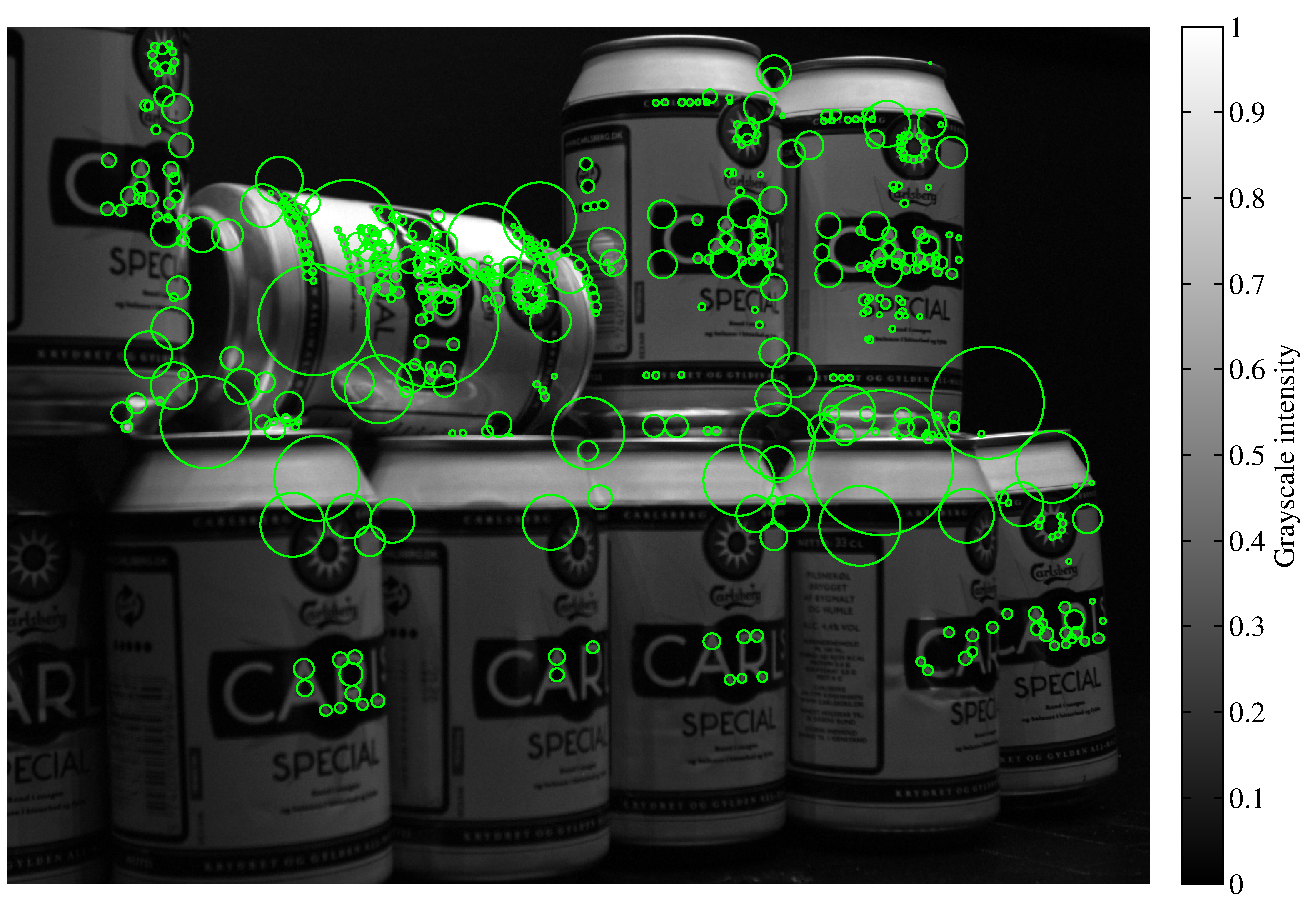
\includegraphics[width=\textwidth]{img/cellHistDetector.pdf}
    \caption{Interest points (green) found by a multi-scale DoG detector on an example image. The circle radii illustrate the detection scale of each point. $529$ points are detected in total.}
    \label{fig:cellHistDetector}
    \vspace{1cm}
    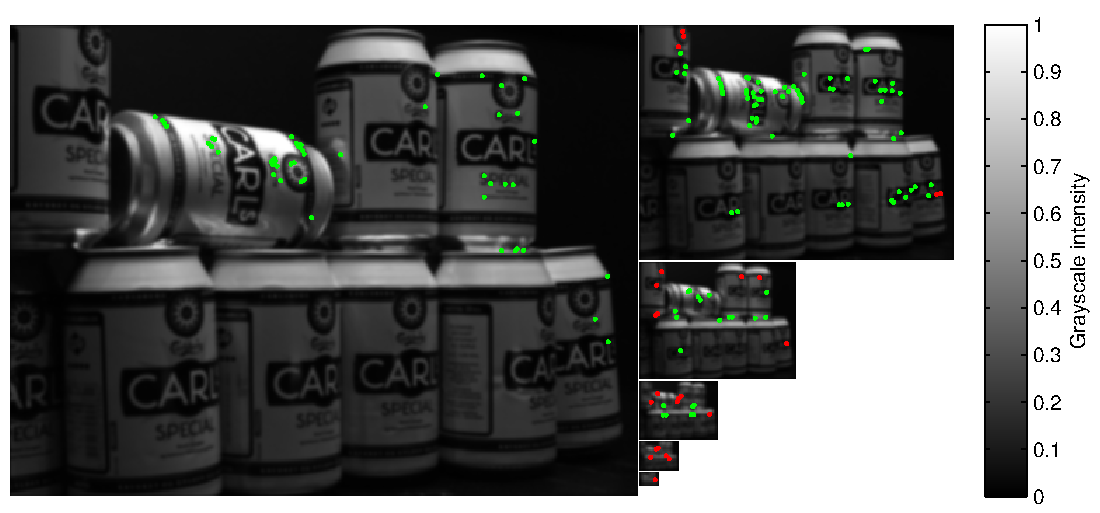
\includegraphics[width=\textwidth]{img/cellHistScaleSpacesP.pdf}
    \caption{The smoothed and downsampled images at various scales with their corresponding kept interest points (green) and removed interest points (red).}
    \label{fig:cellHistScaleSpacesP}
\end{figure}

\begin{figure}[p]
    \centering
    \begin{subfigure}[t]{0.97\textwidth}
		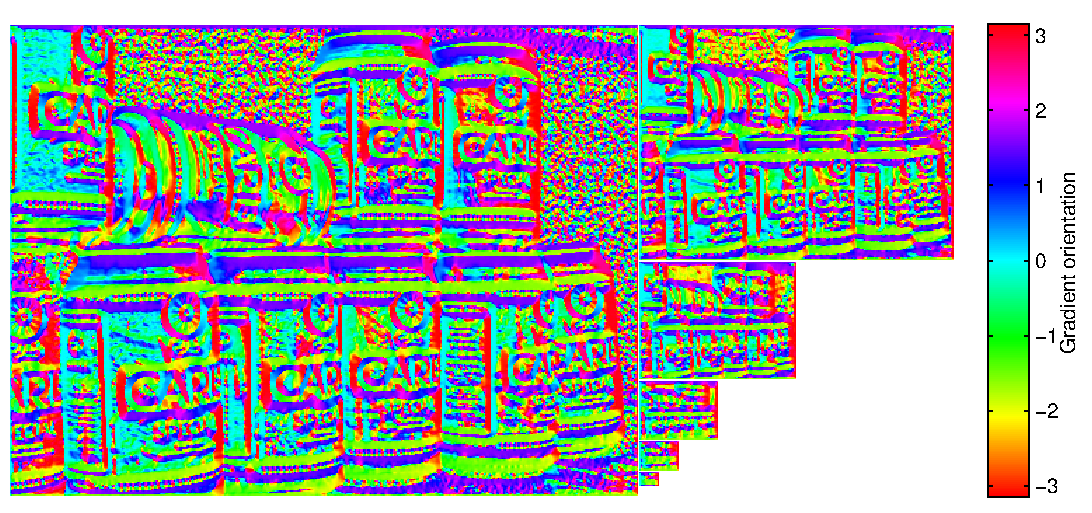
\includegraphics[width=\textwidth]{img/cellHistScaleSpacesV.pdf}
    	\caption{Gradient orientation images }
    	\label{fig:cellHistScaleSpacesV}
	\end{subfigure}
    \begin{subfigure}[t]{0.97\textwidth}
		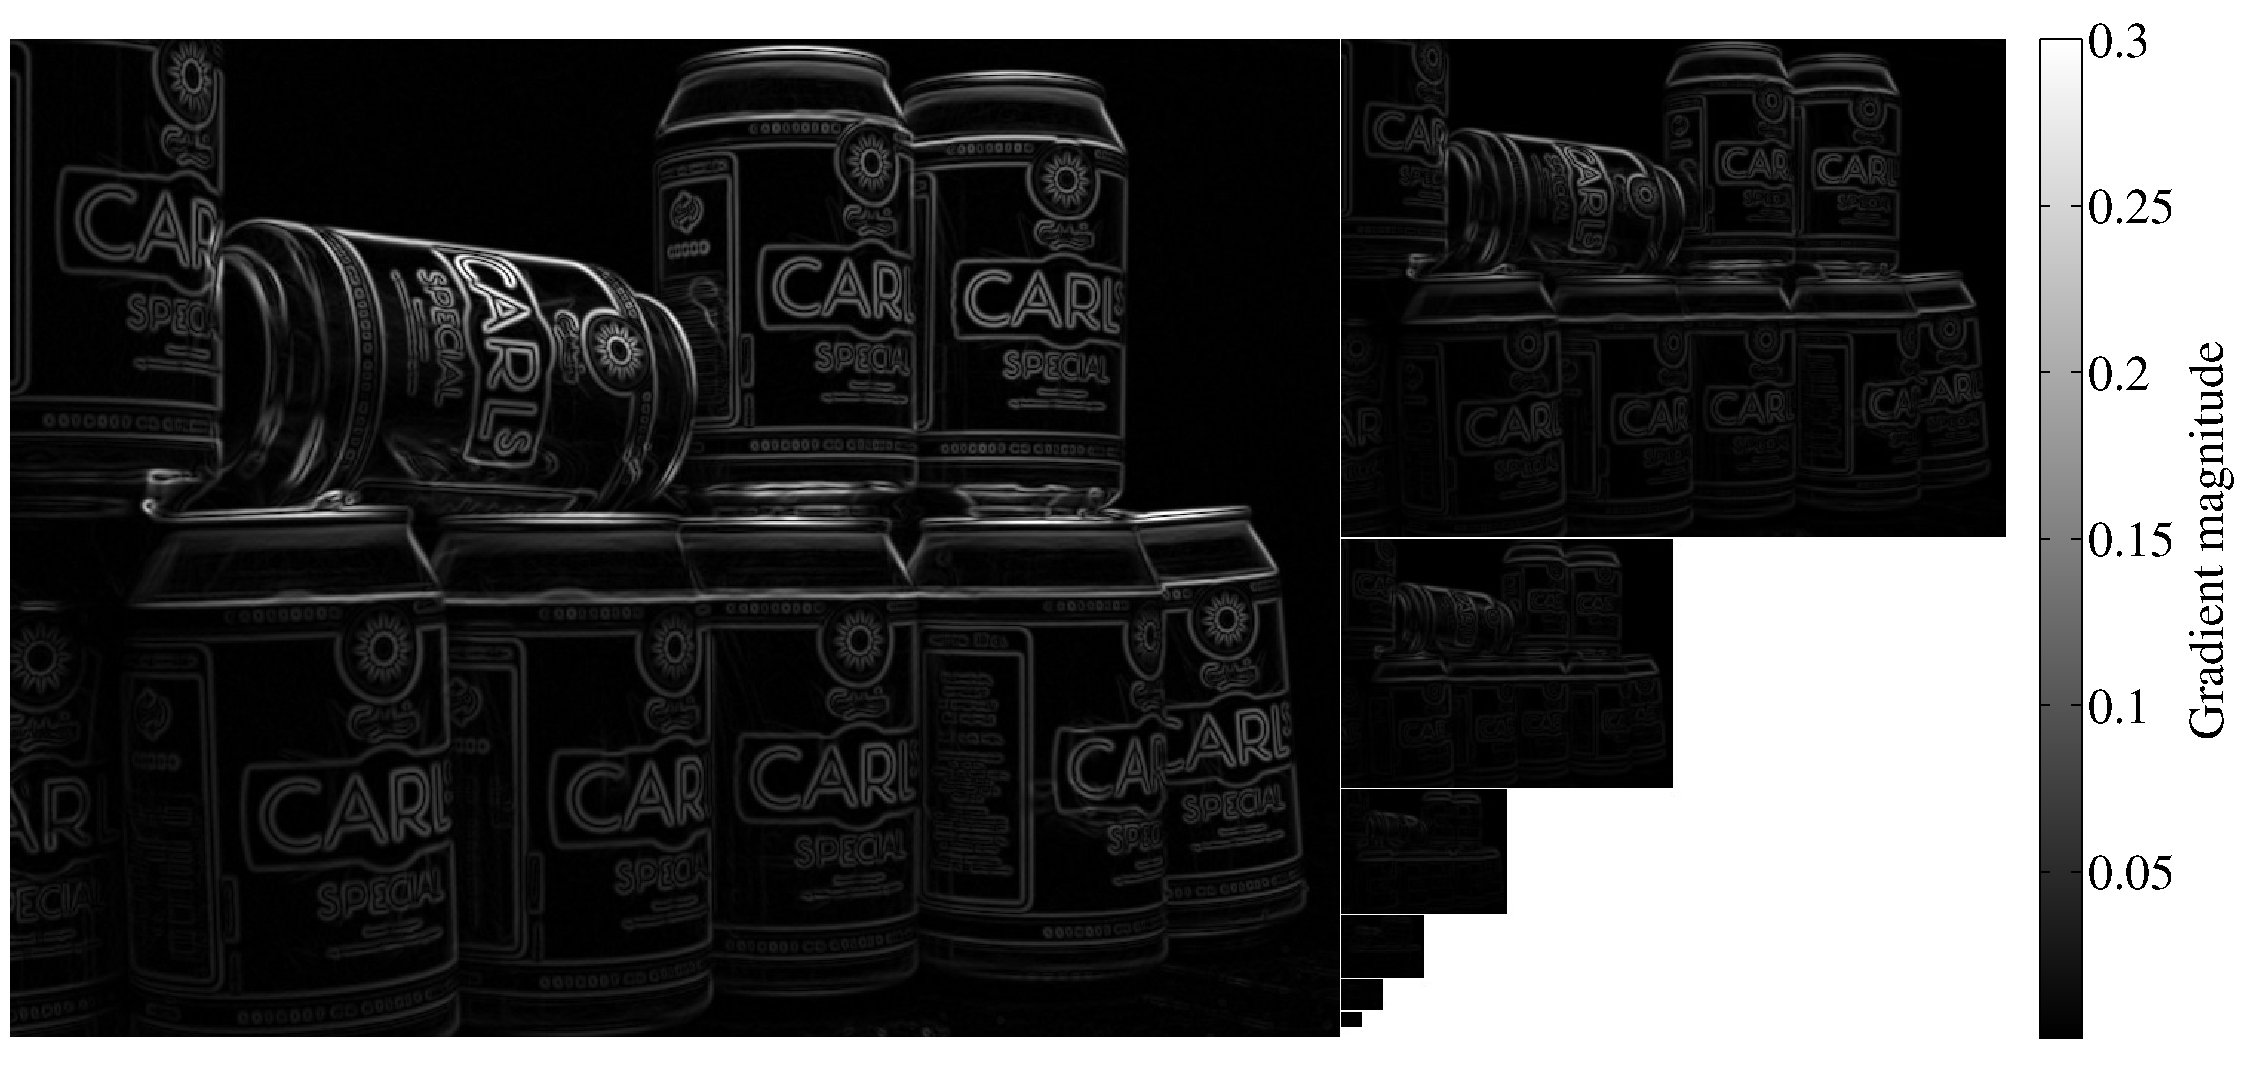
\includegraphics[width=\textwidth]{img/cellHistScaleSpacesM.pdf}
    	\caption{Gradient magnitude images}
    	\label{fig:cellHistScaleSpacesM}
	\end{subfigure}
	\begin{subfigure}[t]{0.97\textwidth}
		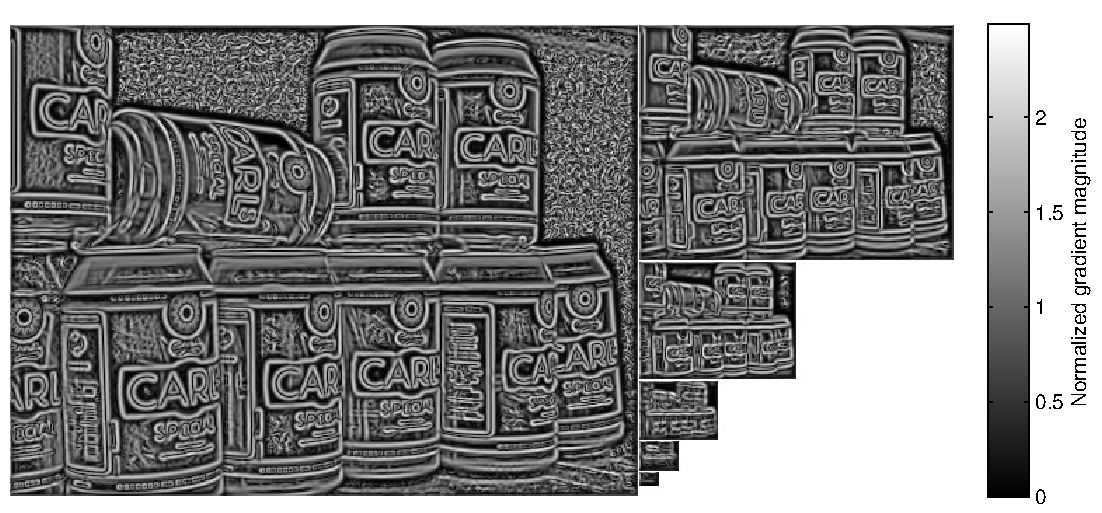
\includegraphics[width=\textwidth]{img/cellHistScaleSpacesMnorm.pdf}
    	\caption{Normalized pixel magnitude images}
    	\label{fig:cellHistScaleSpacesMnorm}
	\end{subfigure}
	\caption{Images \subref{fig:cellHistScaleSpacesV} and \subref{fig:cellHistScaleSpacesM} show gradient orientation and magnitude images computed at various scales. Image \subref{fig:cellHistScaleSpacesMnorm} shows the pixel-wise normalized magnitude images, where the magnitudes are relative to a small local area.}
	\label{fig:cellHistScaleSpacesVM}
\end{figure}

\begin{figure}[p]
    \centering
    \begin{subfigure}[t]{0.97\textwidth}
		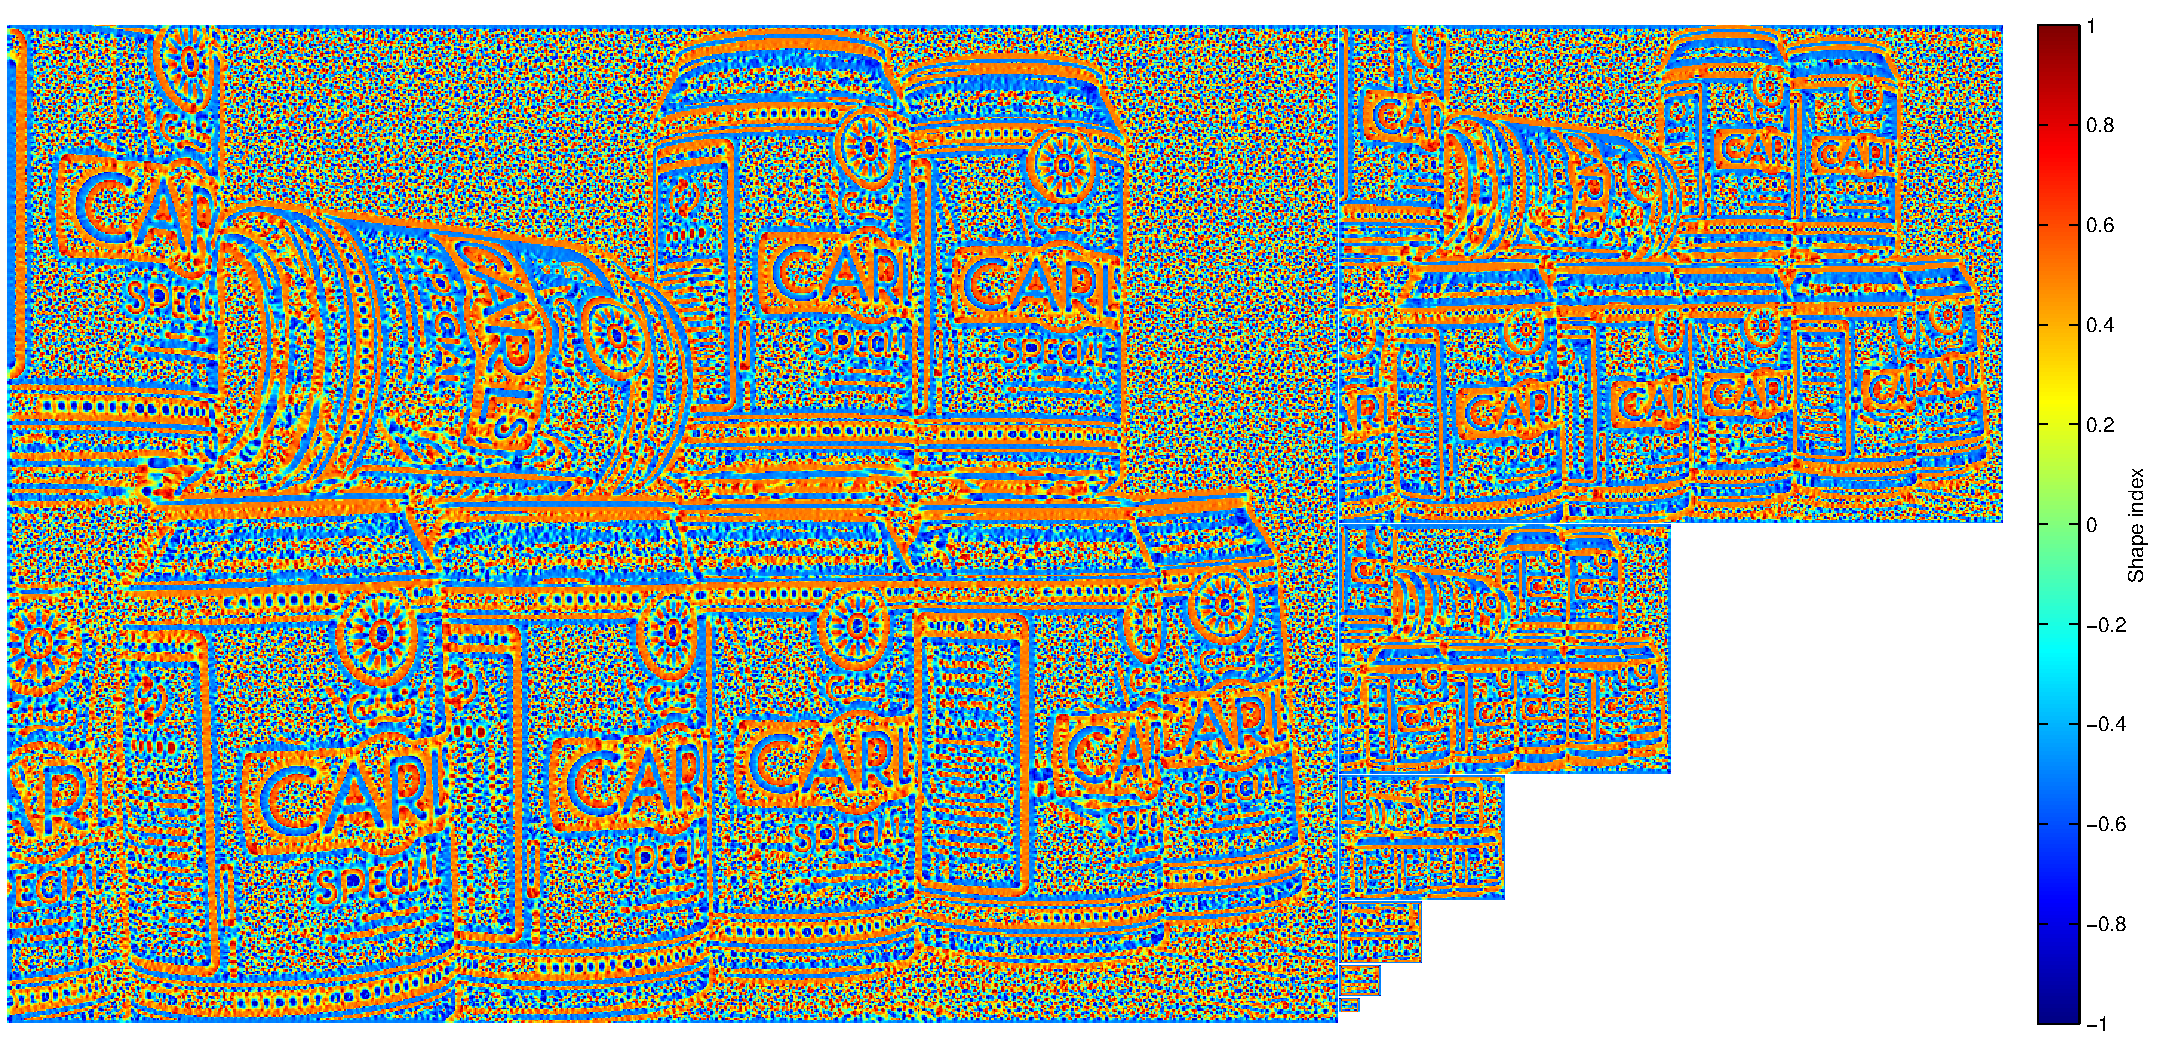
\includegraphics[width=\textwidth]{img/cellHistScaleSpacesS.pdf}
    	\caption{Shape index images}
    	\label{fig:cellHistScaleSpacesS}
	\end{subfigure}
    \begin{subfigure}[t]{0.97\textwidth}
		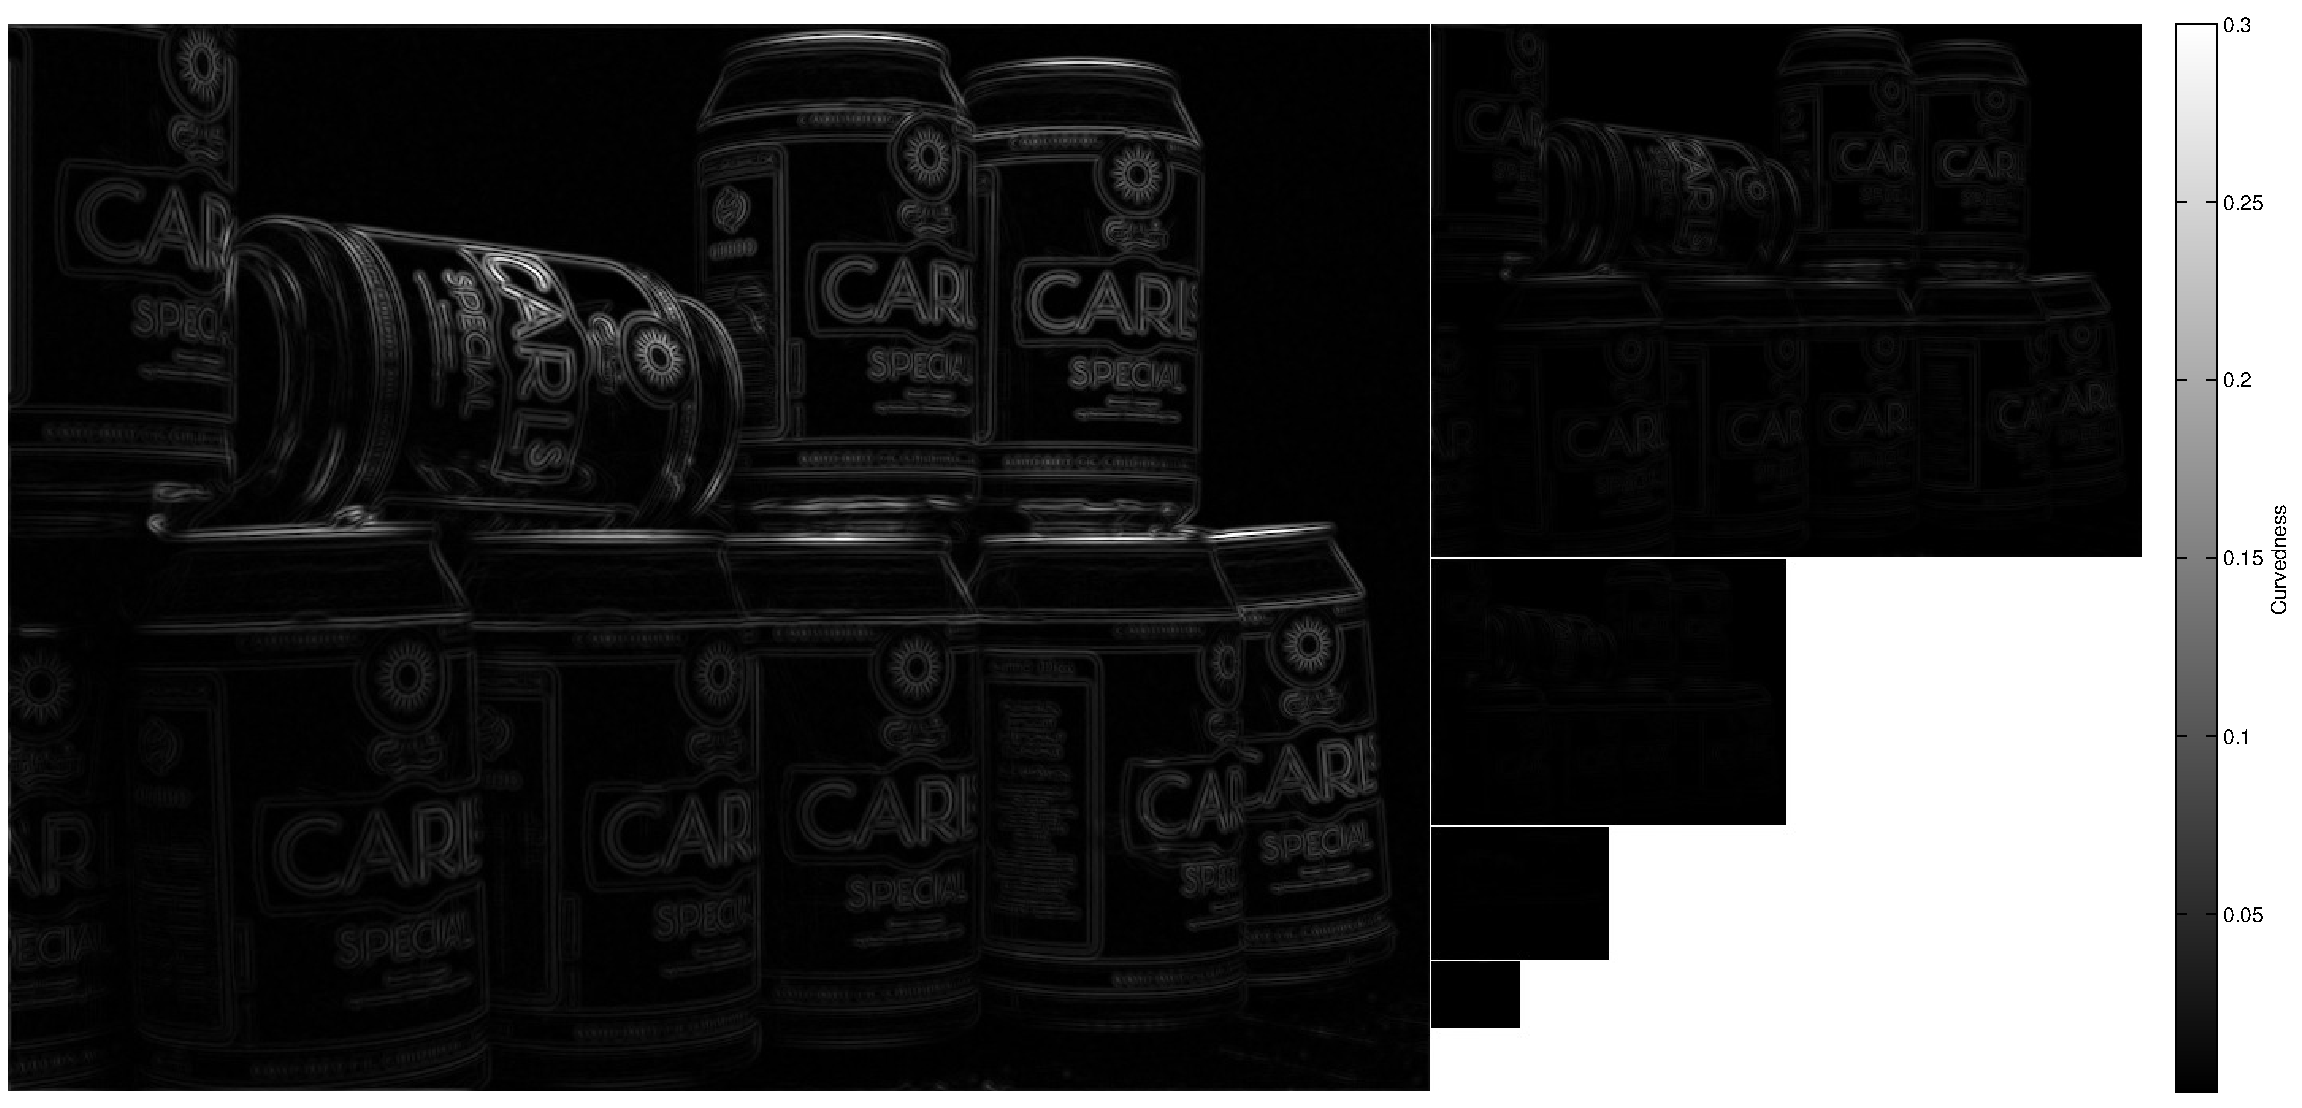
\includegraphics[width=\textwidth]{img/cellHistScaleSpacesC.pdf}
    	\caption{Curvedness images}
    	\label{fig:cellHistScaleSpacesC}
	\end{subfigure}
	\begin{subfigure}[t]{0.97\textwidth}
		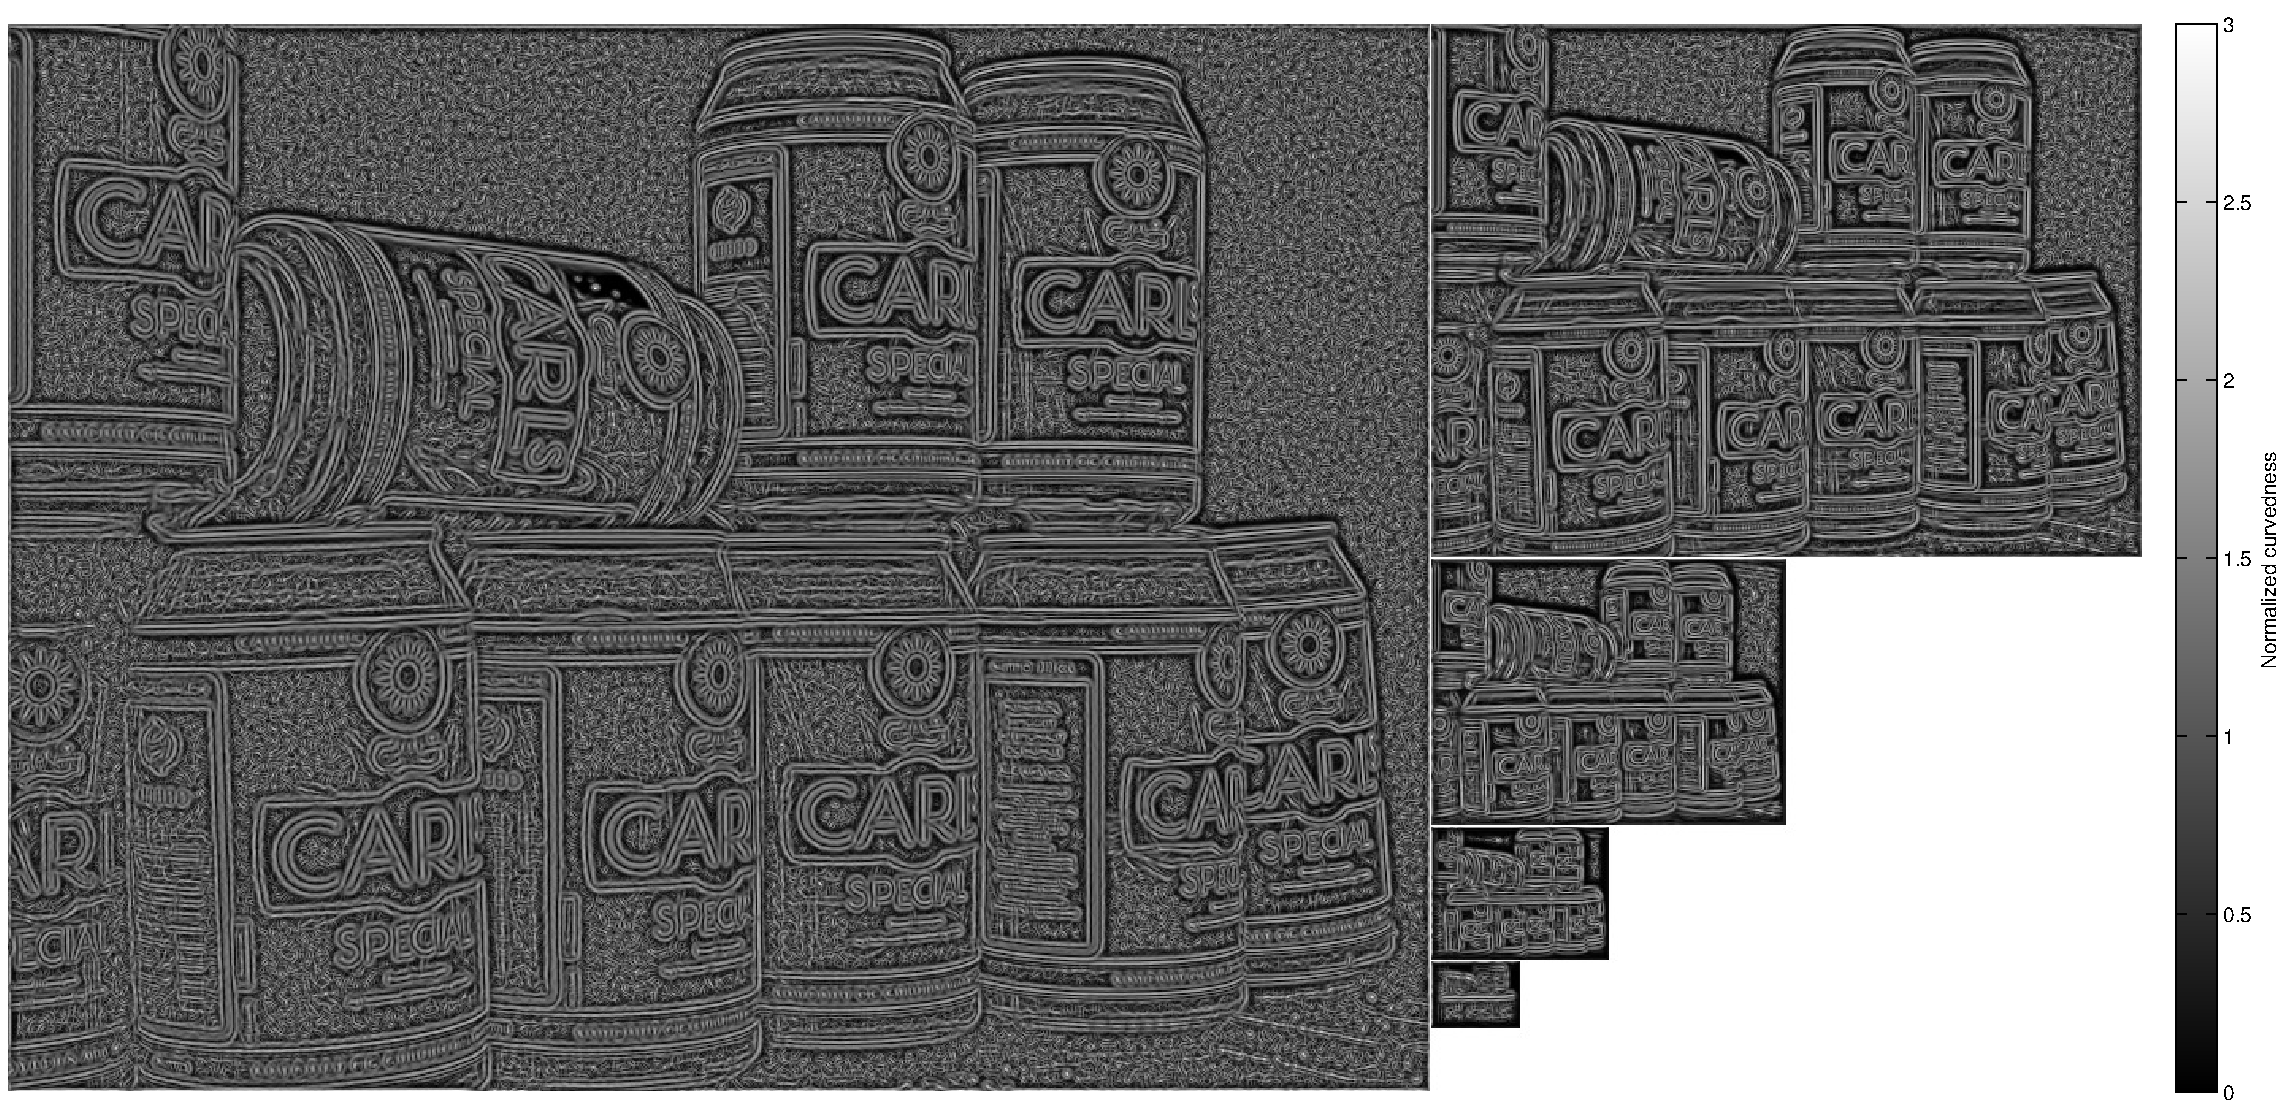
\includegraphics[width=\textwidth]{img/cellHistScaleSpacesCnorm.pdf}
    	\caption{Normalized curvedness images}
    	\label{fig:cellHistScaleSpacesCnorm}
	\end{subfigure}
	\caption{Images \subref{fig:cellHistScaleSpacesS} and \subref{fig:cellHistScaleSpacesC} show shape index and curvedness images computed at various scales. Image \subref{fig:cellHistScaleSpacesCnorm} shows the pixel-ise normalized curvedness images, where the curvedness is relative to a small local area.}
	\label{fig:cellHistScaleSpacesSC}
\end{figure}

From the blurred and downsampled images we apply derivative filters in order to compute value and magnitude images by their respective functions. In the case of GO, $x$- and $y$-derivatives are needed, whereas $xx$-, $xy$-, and $yy$-derivatives are needed for SI. The derivatives are used to compute bin value and magnitude functions over the entire image. We then apply our pixel-wise normalization scheme to the magnitudes\todo{What is $\eta$?}. These images are shown in \Cref{fig:cellHistScaleSpacesVM,fig:cellHistScaleSpacesSC} for GO and SI respectively.

We need to compute the cell and center weights for pixels in every cell according to the chosen cell layout parameters. In this case we use Gaussian cell kernels, where the support radius is confined to $3$ times the cell radius. Pixels outside this distance to each cell center are ignored. For pixels inside, we compute the spatial weights according to \Cref{sec:cellApertureFunction,sec:centerApertureFunction}. The products of these weights are illustrated in \Cref{fig:cellHistScaleSpacesSpatialWeights}, but since many cells overlap we show the maximal weight for each pixel.

The last type of weights needed are the bin values. \Cref{fig:cellHistScaleSpacesBins} shows bin value images for two bin centers with opposite gradient orientations. The purpose of these images is to illustrate the bin weighting and hence we have left out the corresponding SI examples. The images clearly show their corresponding parts of the beer can structures as well as some background noise. Though not shown in these images, to save computation time we only compute bin values once for each pixel with a non-zero spatial weight, and we then simply look up the value when needed in a cell.

Finally, the four weights are multiplied in order to construct the cell histograms. \Cref{fig:cellHistFigureGoM,fig:cellHistFigureSiC} illustrate one of these grids for a single feature for GO and SI respectively. We see that there is a correspondence between the dominating orientations of the GO histograms and the gradient field of the underlying image. The weighted histogram values are then concatenated and normalized for each feature, resulting in the final descriptor. For SI the correspondence between the histograms and the underlying image is harder to see. \todo{Is the figure layout good?}

\begin{figure}[tb]
    \centering
    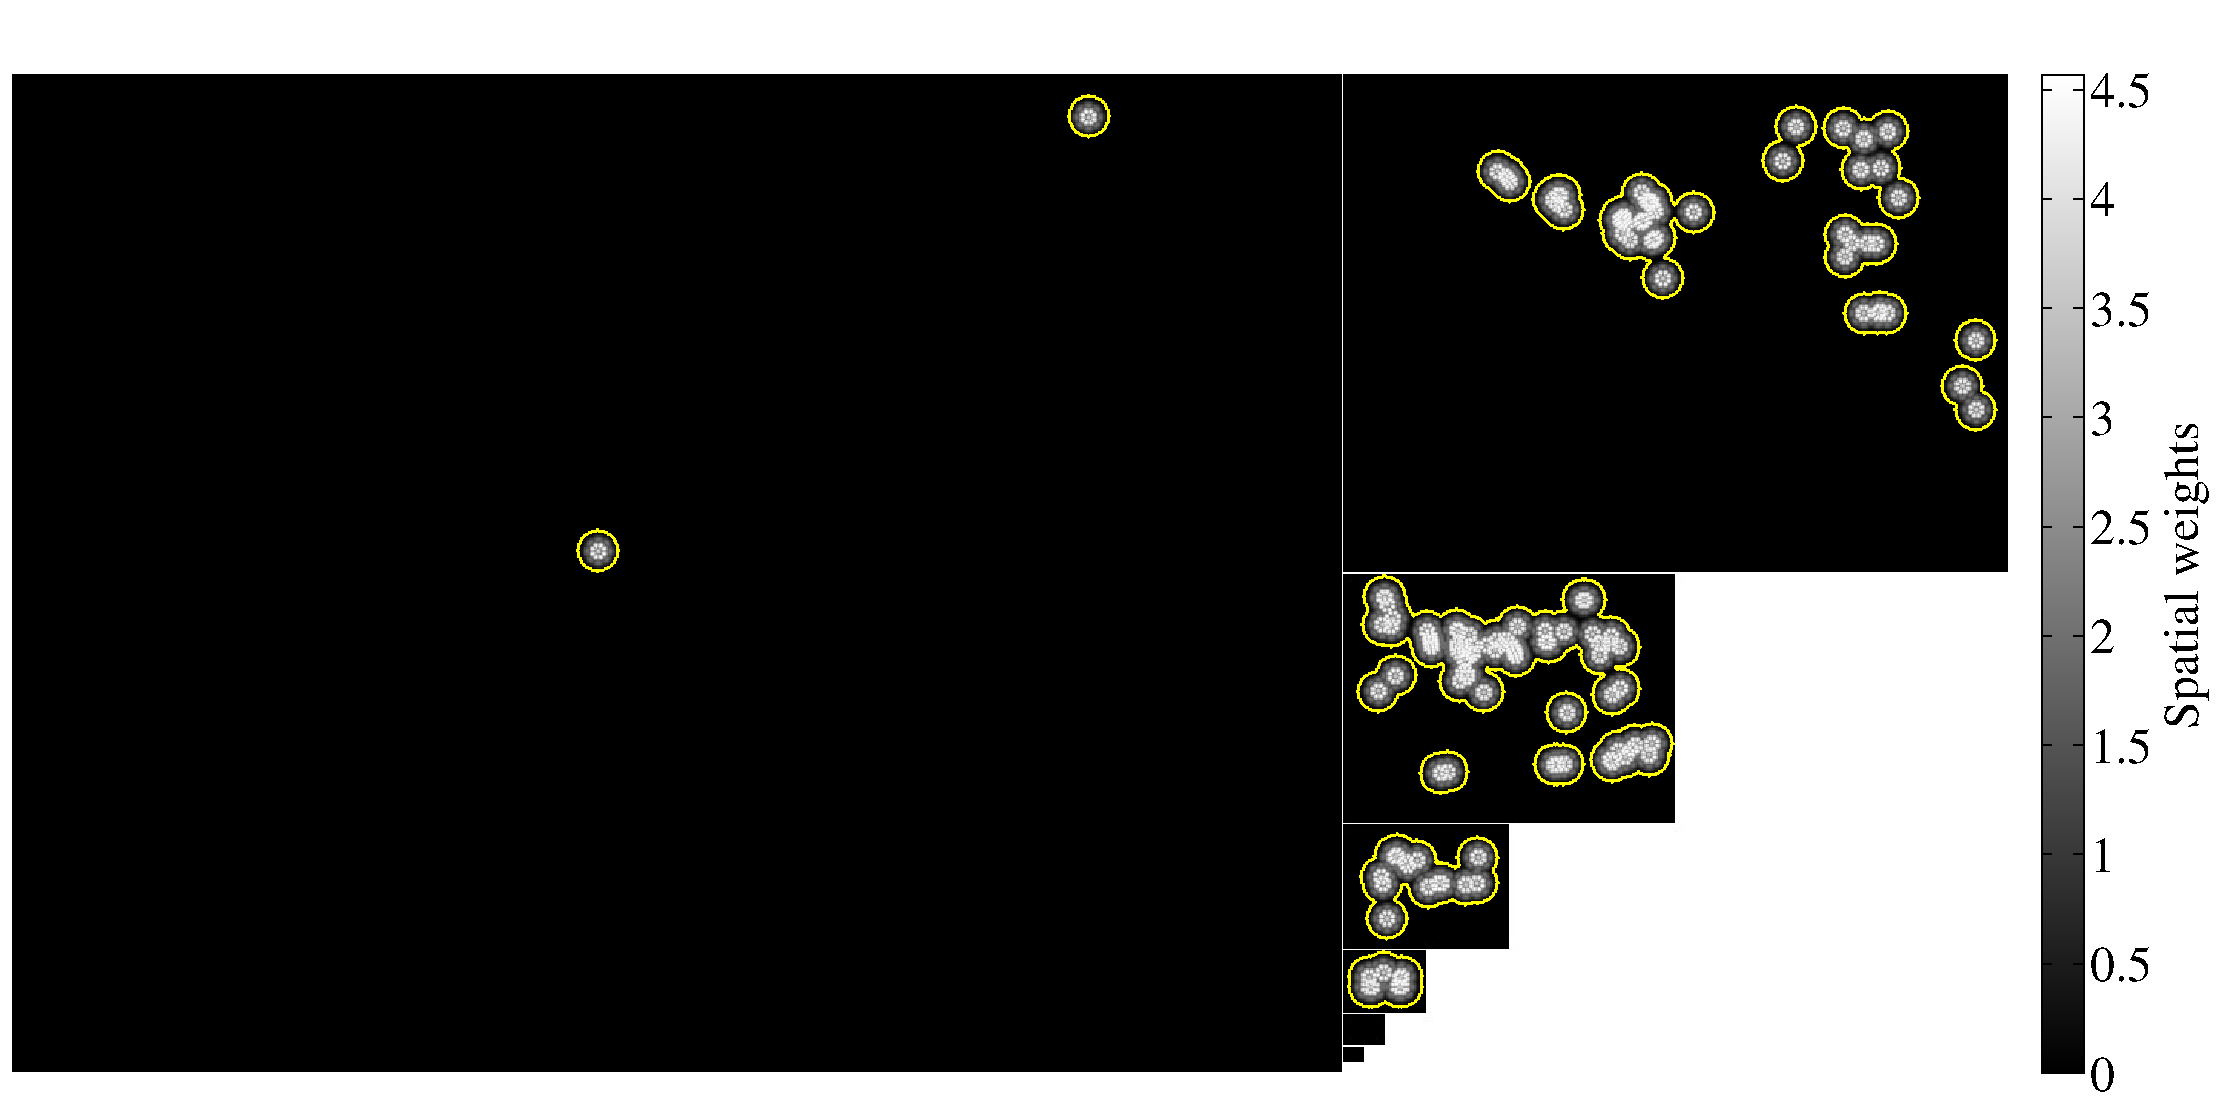
\includegraphics[width=\textwidth]{img/cellHistScaleSpacesSpatialWeights.pdf}
    \caption{Product of cell and center weights. When cells overlap, the maximal weight is shown. The yellow borders indicate the scope of pixels within the support radii of the cells. Only these are used to construct the cell histograms.}
    \label{fig:cellHistScaleSpacesSpatialWeights}
\end{figure}

\begin{figure}[p]
	\centering
	\begin{subfigure}[t]{\textwidth}
		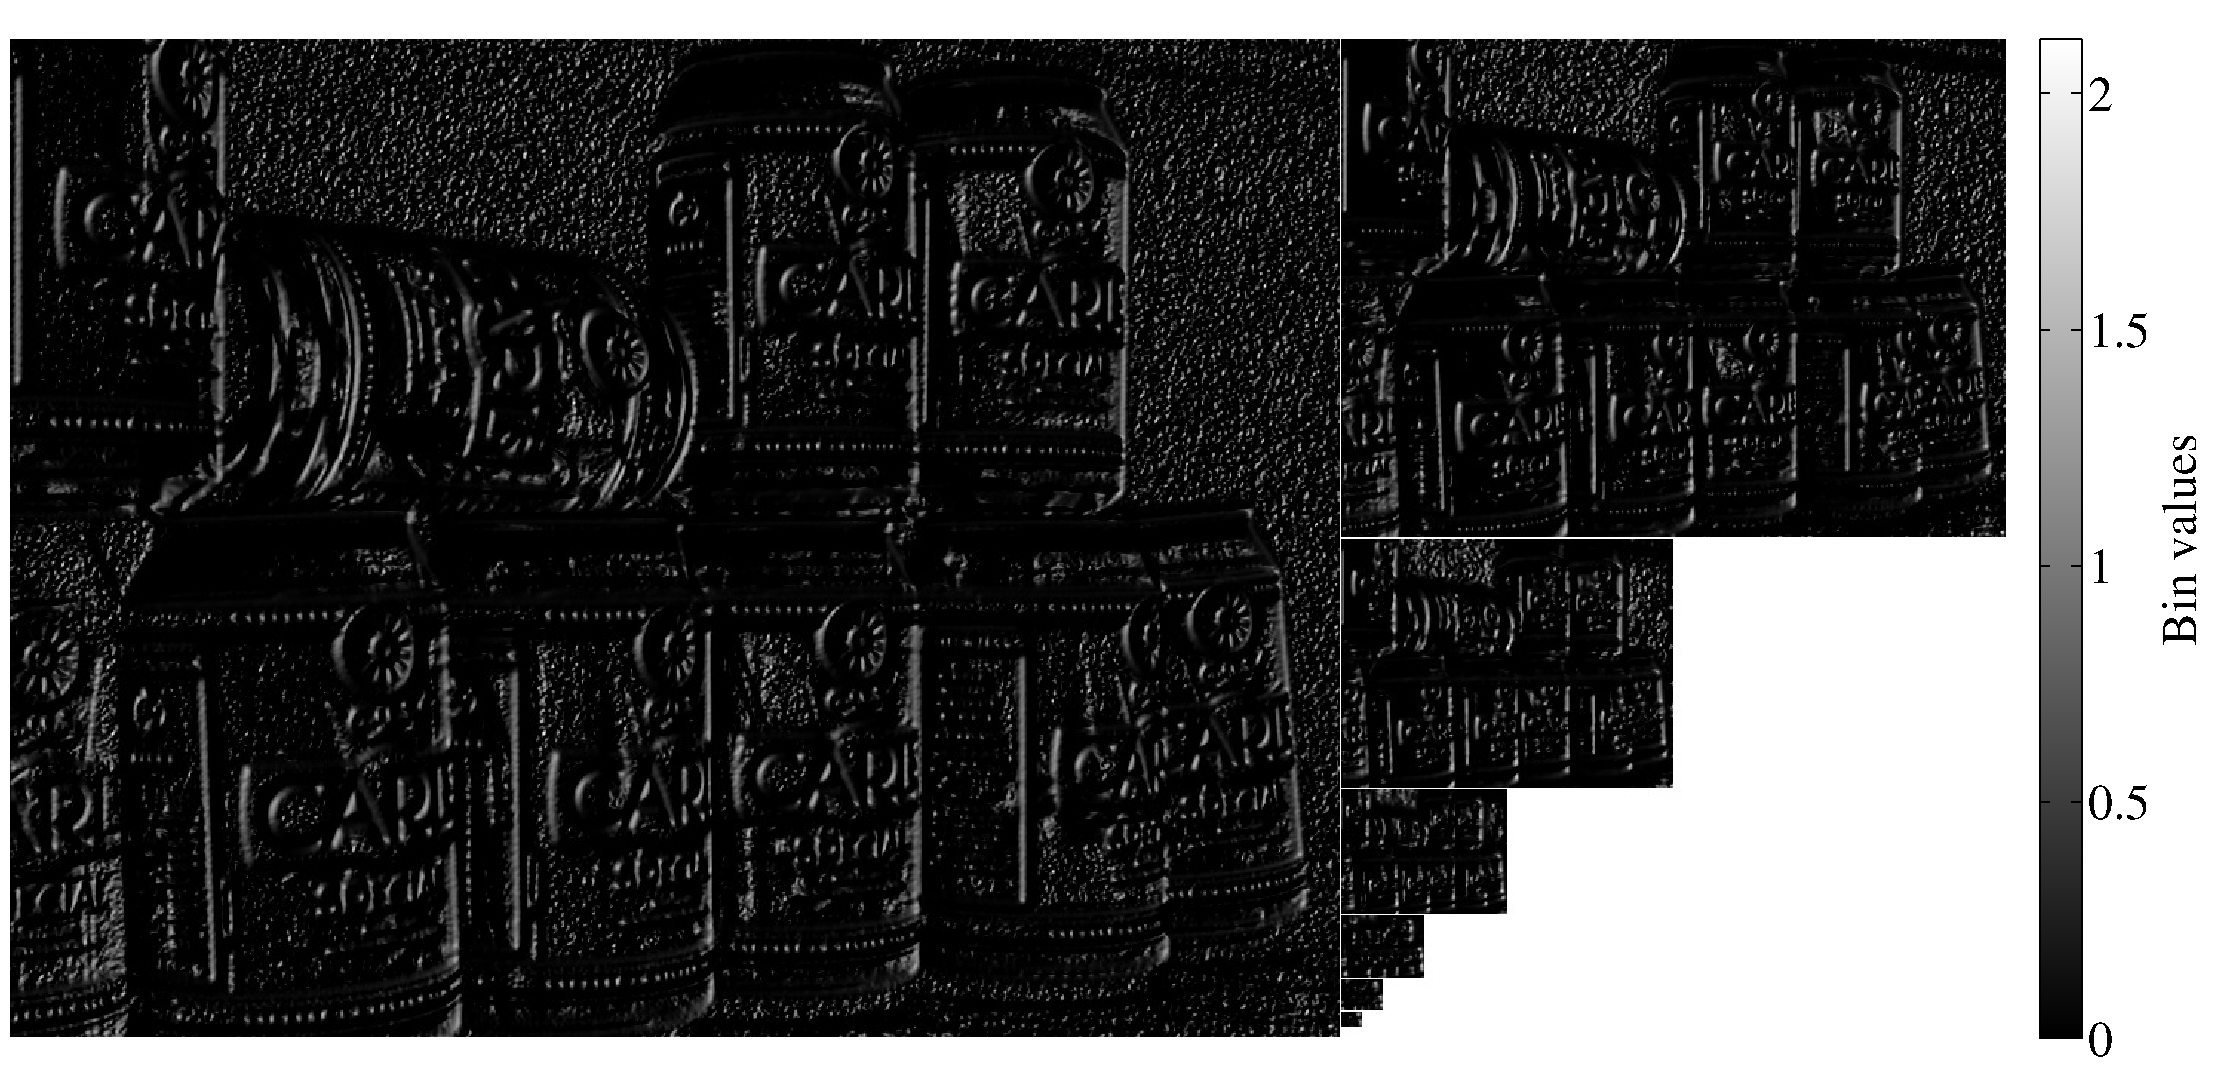
\includegraphics[width=\textwidth]{img/cellHistScaleSpacesBin01.pdf}
    	\caption{Bin $1$ of $8$}
    	\label{fig:cellHistScaleSpacesBin01}
	\end{subfigure}
	\begin{subfigure}[t]{\textwidth}
		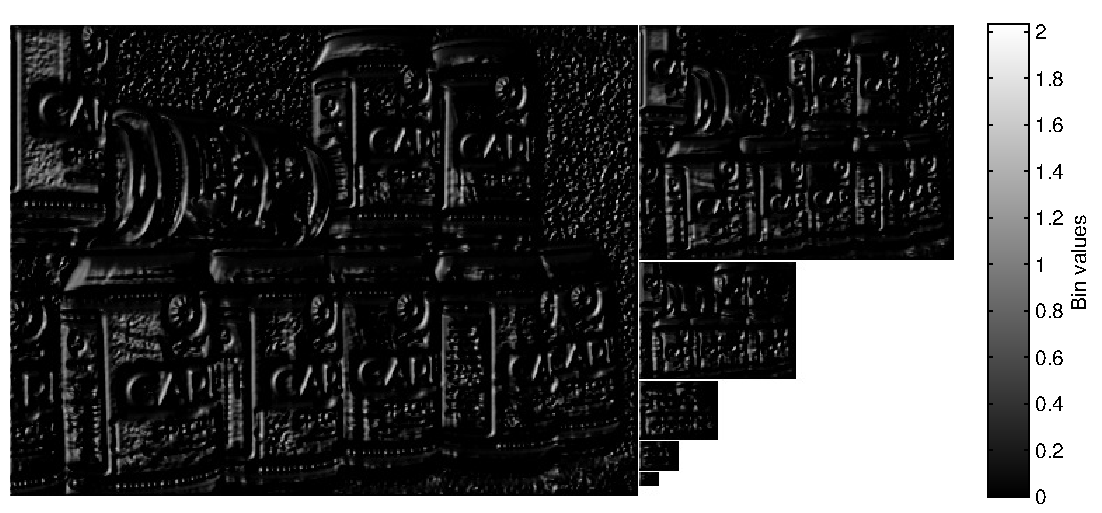
\includegraphics[width=\textwidth]{img/cellHistScaleSpacesBin05.pdf}
    	\caption{Bin $5$ of $8$}
    	\label{fig:cellHistScaleSpacesBin05}
	\end{subfigure}
	\caption{Bin value images for two of the histogram bins. Images \subref{fig:cellHistScaleSpacesBin01} and \subref{fig:cellHistScaleSpacesBin05} correspond to the opposite bin centers $\Theta = -157.5^\circ$ and $\Theta = 22.5^\circ$, and we see that opposite sides of the beer cans are given the greatest bin values for each image.}
	\label{fig:cellHistScaleSpacesBins}
\end{figure}

\begin{figure}[tb]
    \centering
    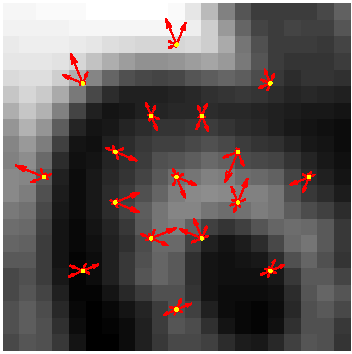
\includegraphics[width=0.65\textwidth]{img/cellHistFigureGo.pdf}
    \caption{The cell histograms for a single feature that make up our GO descriptor. For each cell center (yellow), the weighted histogram values (red) are drawn in the direction of the corresponding bin center orientations. We see that the cell histograms generally point towards larger intensities.}
    \label{fig:cellHistFigureGoM}
\end{figure}

\begin{figure}[p]
   	\centering
	\begin{subfigure}[t]{0.65\textwidth}
	    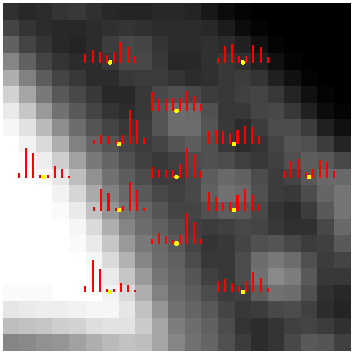
\includegraphics[width=\textwidth]{img/cellHistFigureSi.pdf}
	    \caption{}
   	    \label{fig:cellHistFigureSiCfeature}
    \end{subfigure}
    \begin{subfigure}[t]{0.65\textwidth}
    	\centering
    	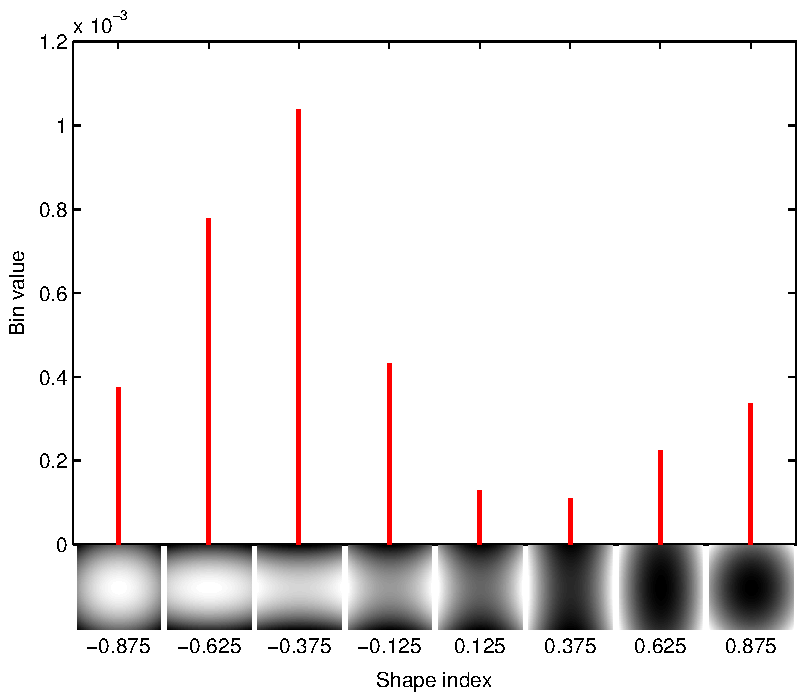
\includegraphics[width=\textwidth]{img/cellHistFigureSiExample.pdf}
%   	\end{subfigure}
%   	\begin{subfigure}[t]{0.1\textwidth}
		\caption{}
		\label{fig:cellHistFigureSiChist}
   	\end{subfigure}
   	\caption{The cell histograms for a single feature that make up our SI descriptor \subref{fig:cellHistFigureSiCfeature}. For each cell center (yellow), the weighted histogram values (red) are drawn. \subref{fig:cellHistFigureSiChist} illustrates the central histogram of \subref{fig:cellHistFigureSiCfeature} where the images at each bin show examples of the corresponding structure.}
    \label{fig:cellHistFigureSiC}
\end{figure}
%
\subbibliography

\end{document}
